\documentclass[12pt]{article}
\usepackage[utf8]{inputenc}

% Importing settings from setup.sty
\usepackage{setup}
\usepackage{booktabs}
\usepackage{multicol}
\usepackage{multirow}
\usepackage{tikz}
\usetikzlibrary{shapes.geometric, shapes.multipart, arrows, positioning}
\tikzstyle{data} = [ellipse, minimum width=1cm, minimum height=1.2cm,text centered, draw=black, fill=blue!20]
\tikzstyle{preprocessing_container} = [rectangle split,rectangle split parts=7, rectangle split draw splits=false, rounded corners, text width=12cm, minimum height=5cm, draw=black, fill=orange!20]
\tikzstyle{preprocessing} = [rectangle, rounded corners, minimum width=3cm, minimum height=1cm, draw=black, fill=orange!50]
\tikzstyle{classifier} = [rectangle, rounded corners, minimum width=3cm, minimum height=1cm, text centered, draw=black, fill=magenta!30]
\tikzstyle{result} = [rectangle, minimum width=3cm, minimum height=1cm, text centered, draw=black, fill=green!40]
\tikzstyle{arrow} = [thick,->,>=stealth]


% \pagenumbering{roman}
\begin{document}


% Inserting title page
\import{./}{title}


\pagenumbering{roman}
\tableofcontents
\listoffigures
\listoftables

% \restoregeometry
\newgeometry{
    left=25mm,
    right=25mm,
    top=25mm,
    bottom=25mm}
\pagenumbering{arabic}

\section{Problem description}
The problem we are trying to solve consists of predicting whether an animal will be adopted from a shelter within 30 days, given several pieces of information on this animal. This problem is a clean and reduced version of a \href{https://www.kaggle.com/c/petfinder-adoption-prediction/overview}{Kaggle competition} dating back from 2019.

\section{Exploratory Data Analysis}
We would like to get some basic information of the data set before diving into the machine learning solution. \\
The training set has shape \((8168 \times 16)\) and the test set has shape \((250 \times 16)\), where the column names and data types are summarized in Table \ref{table: column data type}. \\
\begin{table}[!ht]
    \centering
    \begin{tabular}{ccccc}
        % \textbf{Type}                       &  & \multicolumn{1}{c}{\textbf{Column name}} \\ \midrule
        \toprule
        \multicolumn{2}{c}{\textsc{categorical}} & \textsc{numerical} & \textsc{text} & \textsc{image}          \\ \midrule
        Type                                     & MaturitySize       & Age           & Description    & Images \\
        Gender                                   & FurLength          & Fee                                     \\
        Breed                                    & Vaccinated                                                   \\
        Color1                                   & Dewormed                                                     \\
        Color2                                   & Sterilized                                                   \\
        Color3                                   & Health                                                       \\
        \bottomrule
    \end{tabular}
    \caption{Data types per column}
    \label{table: column data type}
\end{table} \\
Overall, the data set is very clean as it contains 0 NaN values.




\section{Solution}
The solution consists of a pipeline of the following structure:

\begin{center}
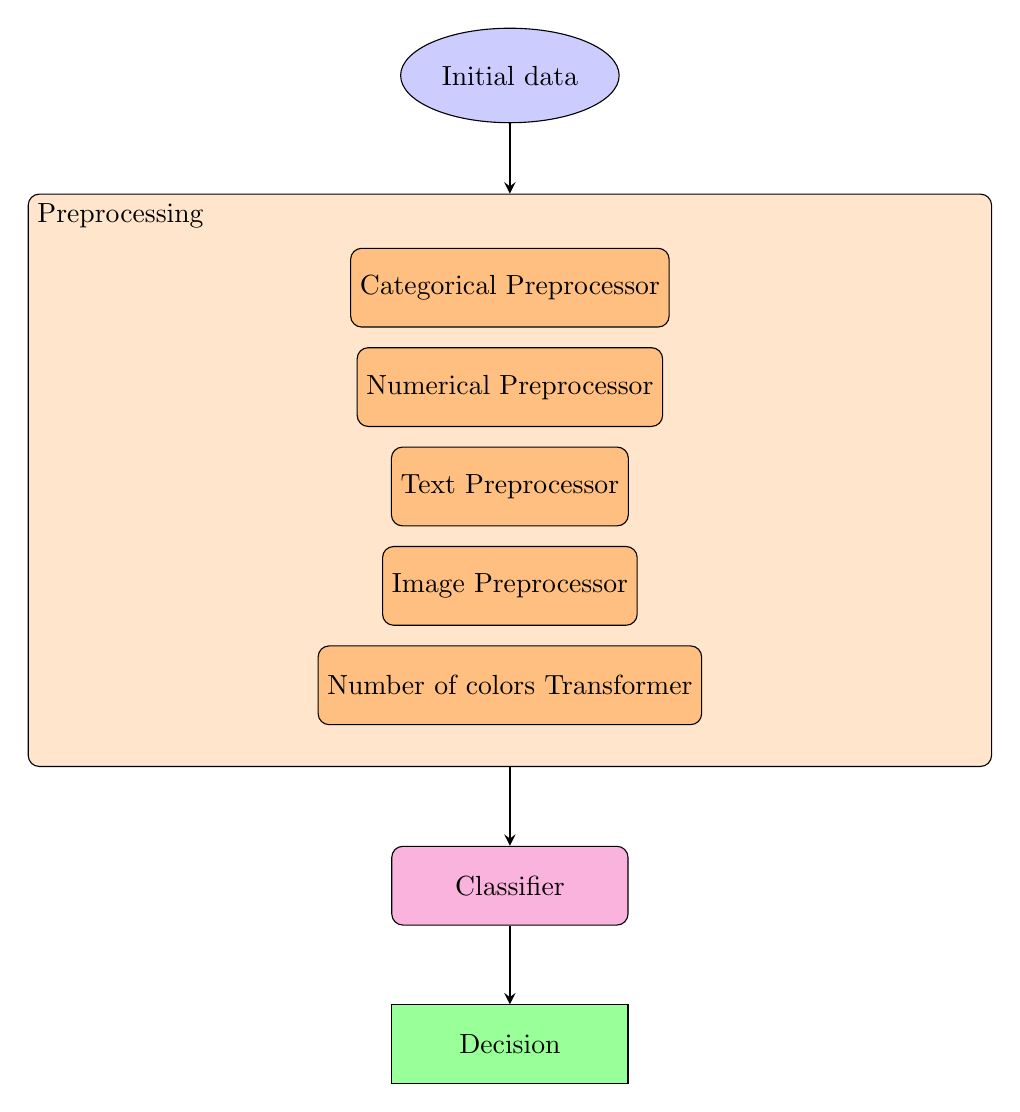
\begin{tikzpicture}[node distance=1.5cm]
    \node (start) [data] {Initial data};
    \node [align=center](preprocessing_container) [preprocessing_container, below of=start, anchor=north] {
        \nodepart[align=left]{one}Preprocessing
        \nodepart{two}
        \tikz{\node (categorical_preprocessor) [preprocessing] {Categorical Preprocessor}}
        \nodepart{three}
        \tikz{\node (numerical_preprocessor) [preprocessing] {Numerical Preprocessor}}
        \nodepart{four}
        \tikz{\node (text_preprocessor) [preprocessing] {Text Preprocessor}}
        \nodepart{five}
        \tikz{\node (image_preprocessor) [preprocessing] {Image Preprocessor}}
        \nodepart{six}
        \tikz{\node (nb_colors) [preprocessing] {Number of colors Transformer}}
    };
    \node (classifier) [classifier, below=1cm of preprocessing_container, anchor=north] {Classifier};
    \node (result) [result, below=1cm of classifier, anchor=north] {Decision};

    \draw [arrow] (start) -- (preprocessing_container);
    % \draw [arrow] (preprocessing_container.two) -- (preprocessing_container.three);
    % \draw [arrow] (numerical_preprocessor) -- (text_preprocessor);
    % \draw [arrow] (text_preprocessor) -- (image_preprocessor);
    % \draw [arrow] (image_preprocessor) -- (nb_colors);
    % \draw [arrow] (nb_colors) -- (result);
    \draw [arrow] (preprocessing_container) -- (classifier);
    \draw [arrow] (classifier) -- (result);
\end{tikzpicture}
\end{center}



\begin{table}[!ht]
    \centering
    \begin{tabular}{ccc}
        \toprule
        \textbf{Classifier}        & \textbf{Accuracy} \\ \midrule
        GradientBoostingClassifier & 0.629             \\
        RandomForestClassifier     & 0.623             \\
        AdaBoostClassifier         & 0.612             \\
        MLPClassifier              & 0.602             \\
        BernoulliNB                & 0.600             \\
        GaussianNB                 & 0.567             \\
        DecisionTreeClassifier     & 0.559             \\
        SVC                        & 0.529             \\
        KNeighborsClassifier       & 0.520             \\
        GaussianProcessClassifier  & 0.509             \\
        SGDClassifier              & 0.509             \\ \bottomrule
    \end{tabular}
    \caption{Accuracies of first prospect}
\end{table}
We did not test XGBoost because is too slow.

\section{Evaluation \& critical view}

\end{document}